\documentclass[a4paper,12pt]{article}
%\usepackage[utf8]{inputenc}
\usepackage{graphicx}
%\usepackage[magyar]{babel}
%\usepackage{t1enc}

\begin{document}

\author{Istvan Elek}

\title{Giwer's Users' Guide}


\date{\today}


\setcounter{tocdepth}{3}
%\frontmatter
\maketitle
\newpage
\tableofcontents
\newpage
%\mainmatter


\section{Introduction}

There are some open and commercial image processing system which can be applied to drone images such as ENVI, ArcGIS, SAGA, QGIS etc. They have many high level image processing skills, but if you attempt to implement your special algorithm the task can become difficult or impossible. It was the initial conception for developing Giwer.
The developers' purpose was:

\begin{enumerate}
	\item Create a system suitable for processing images made from space and air
	\item Make it possible to process multiple images in batch mode like a project
	\item The system should also be able to process images made by not only a drone but any satellite or aircraft
	\item Users can create their own workflows from the functions available in Giwer, consequently your batch processes become tailor-made
	\item Let Giwer be open source with GNU3 licence thus the executable and the source files can be reached
\end{enumerate}

\subsection{Installation}

\begin{enumerate}
	\item Create an appropriate folder where you want giwer be (e.g. D:\\giwer)
	\item Download the giwer.zip file and save it to this folder
	\item Unzip
	\item Let us start (click to giwer.exe)
\end{enumerate}

\section{The frame program}

We have developed the program pack in C\# that handles, processes and analyses many image formats (bil, tif, geotif, jpg).
The name of the frame program is Giwer.  It organizes the different components, such as Catalog, DataStock, WorkflowBuilder, Config (config viewer/editor), Help (users’ guide) and Info (information on the Giwer system).  Let us look at one after the other. To start the frame program click to \textit{giwer.exe} (fig. \ref{fig:giwerMain}).


\begin{itemize}
	\item It organizes the raw images into a database (Sqlite), which extracts number of data describing a certain image from its exif data, and also provides storage options in interactive fields (\textbf{Catalog}).
	\item We have implemented a large number of image processing functions, which can be accessed through a menu system, interactively (\textbf{DataStock})
	\item From the available functions, arbitrary workflows can be compiled, so the user can create his own processing procedures (\textbf{WorkflowBuilder}) based on his individual knowledge, experience and creativity.
\end{itemize}

	\begin{figure}
	\centering
	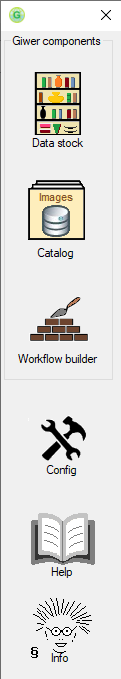
\includegraphics[width=2cm]{giwerMain.png}
	\caption{The GUI of the frame program}
	\label{fig:giwerMain}
\end{figure}


Every subsystem can be launched individually or from the frame program.

\subsection{Giwer’s processing abilities}

There is a frame program which organizes the available subsystems (DataStock, Catalog, WorkflowBuilder), launched them, set up programs' parameters, data sources etc. and save them into a config file. The following modules are available:
\begin{itemize}
	\item DataStock: an interactive image processing and interpretation software package
	\item Catalog: organizes large amounts of images and stores their attributes in a database
	\item WokflowBuilder: Workflow editor and launcher
	\item Config: configure the system (fig. \ref{fig:config})
			
	\begin{figure}
		\centering
		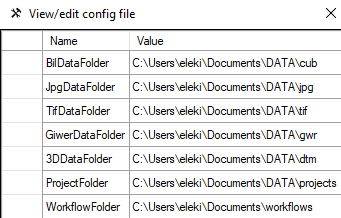
\includegraphics[width=4cm]{config.png}
		\caption{A \textbf{Config} viewer/editor}
		\label{fig:config}
	\end{figure}

	\item Help: Users' guides and tutorials
	\item Info: general information about Giwer and authors
\end{itemize}

%\begin{figure}
%	\centering
%	
\includegraphics[width=12cm]{giwer.png}
%	\caption{The GUI of the frame program }
%	\label{fig:giwer}
%\end{figure}

\section{Catalog}

\textbf{Catalog} is an SQLite-based program for storing and systematizing the attributes of images. It allows you to import freshly taken images directly from the drone's media, read their attribute and position data, and store them in an \textit{SQLite} data file. We can store data interactively not only from the EXIF data of the image. Even a deployment report can be created/edited if needed. An Sql command editor helps you find the images you need.
Let us start working.

\begin{itemize}
	

\item At the first start, there is no image database yet, so \textbf{Catalog} will complain about its lack (fig. \ref {fig:missingdb}): 

\begin{figure}
	\centering
	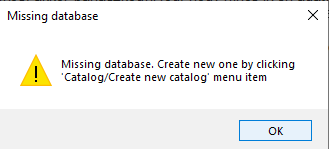
\includegraphics[width=8cm]{missingdb.png}
	\caption{The 'Missing database' message if you start \textbf{Catalog} at first, or the image file catalogue was deleted or moved somewhere}
	\label{fig:missingdb}
\end{figure}

\item Then the main form of the program appears, where you can create a new, empty data file (fig. \ref {fig:createnewcatalog}.) The default name is 'dronimagecatalog.s3db', but you can choose anything else). 

\begin{figure}
	\centering
	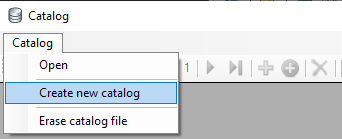
\includegraphics[width=8cm]{createnewcatalog.png}
	\caption{The \textit{Create new catalog} menu}
	\label{fig:createnewcatalog}
\end{figure}

\item Then clicking on the 'Open' menu will open the empty database file. 

\item If an image database already exists (eg as dronimagecatalog), its contents are displayed in a table in the main form of the program (\ref{fig:catalog0}). It's rare, but if it doesn't, you'll complain that there is no such database — because, for example, we've deleted it from the file system, but the \textbf{Catalog} still remembers that there is such a file. Click OK, and then press F2 - around the upper left corner of the keyboard. A menu called 'Catalog' will appear. Select the 'Create new catalog' submenu, which will create a database called 'dronimagecatalog' and an empty data table with the name 'images'. This is where the data of the recorded images will be stored. 

\begin{figure}
	\centering
	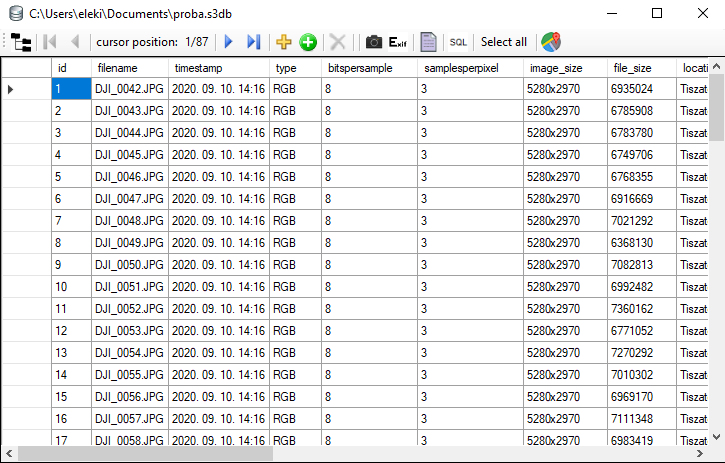
\includegraphics[width=13cm]{catalog0.png}
	\caption{The main form of \textit{Catalog}}
	\label{fig:catalog0}
\end{figure}

\item Menu system is not visible during normal start-up (appears and disappears by pressing F2 key) 

\item The icons ‘tell’ what they know when we move the mouse over them. 
\end{itemize}

\subsection{Preparing the file system }

\begin{itemize}
	\item Create a directory called 'DRON\_IMAGES' somewhere in the file system. 
	
	\item Click on the 'open folder tree' icon 
\includegraphics {open_folder_structure.png}. This will open a window called 'Folder structure' (fig. \ref{fig:folder_struc}). 
	
	\item Click on the menu button named 'Set destination folder', then find and select the directory named 'DRON\_IMAGES'. This will specify the location of image catalogue in the file system, which will be remembered from now on when we reopen the 'Folder structure' window.  
	
	\item Find the directory on the flash drive (which stores the images on the board of drone) where the images you just took are. If the files appear in the right pane, click 'Save files to' \verb|c:\DRON_IMAGES| folder 'icon 
\includegraphics{save.png}. As a result, the contents of the entire folder are copied from the flash drive to the directory named 'DRON\_IMAGES'. 
	
	\item This will cause a new directory to appear in the directory named 'DRON\_IMAGES' which name is the date of first file. This directory will contain images of the flight at that time. 
	
\end{itemize}

\begin{figure}
	\centering
	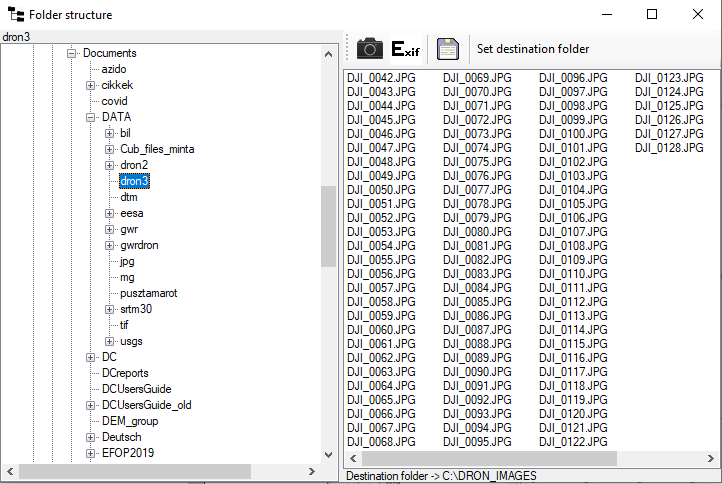
\includegraphics[width=13cm]{folder_struc.png}
	\caption{The \textit{Folder structure} window}
	\label{fig:folder_struc}
\end{figure}

\subsection{Data upload }

\begin{itemize}
	\item There are two ways to upload a database: files individually (or with a multiple file select) or an entire directory, its entire contents (jpg and tif files only, others not). Click on the icon 
\includegraphics [width = 0.5cm] {plus.png} to select per file, or on the icon 
\includegraphics [width = 0.5cm] {addfolder.png} to select the entire directory.
	
	\item Clicking on any of them will bring up a window called 'Editable image attributes' (fig. \ref{fig:editableimageattribute}). The rest of the data is uploaded automatically (file name, longitude, latitude, timestamp, folder, etc.). 
	
	\begin{figure}
		\centering
		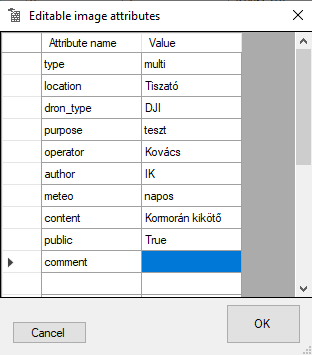
\includegraphics[width=6cm]{editableimageattributes.png}
		\caption{The \textit{Editable image attributes} window}
		\label{fig:editableimageattribute}
	\end{figure}
	
	\item Non-automatic data in the table can be edited, which is saved as soon as we move to the next record. 
	
	\item Clicking on the camera icon 
\includegraphics [width = 0.5 cm] {camera.png} will display the image for the current record. The icon 
\includegraphics [width = 0.6 cm] {exif.png} shows the exif data of the image for the current record in a separate window. 
\end{itemize}

\subsection{Further functions}

Above the table showing the data is an iconostasis on which the main functions are placed. The 
\includegraphics [width = 0.5 cm] {filesystem.png} icon opens a file system view window where you can browse the source of the data, such as a flash drive, which is the data storage device of the drone directly and which contains the latest measurement data (\ref{fig:folder_struc}.). Copy the selected files (the entire directory) to the directory \textit{DRON\_IMAGES}. Anyway, this must be specified the first time you use it (\textit {Set destination folder}). Copying is done by clicking on the 
\includegraphics [width = 0.5cm] {save.png} icon.

Images already in the database can be viewed with the 
\includegraphics [width = 0.5 cm] {camera.png} icon, while the corresponding EXIF data can be viewed with the 
\includegraphics [width = 0.5 cm] {exif.png} icon.

New images can be added to the database individually, with the 
\includegraphics [width = 0.5cm] {plus.png} icon, and in bulk, ie the contents of an entire directory, with the 
\includegraphics [width = 0.5cm] {addfolder.png} icon. The addition icon also uploads the database, of course only the data that can be extracted from the images. You can also add data interactively by entering it in the appropriate field. 

Use the 
\includegraphics [width = 0.5cm] {del.png} icon to delete a selected record. Not only the descriptive data is deleted (the selected record in the table named 'images'), but also the selected image file from the \textit {DRON\_IMAGES} directory (no UNDO). 

\begin{figure}
	\centering
	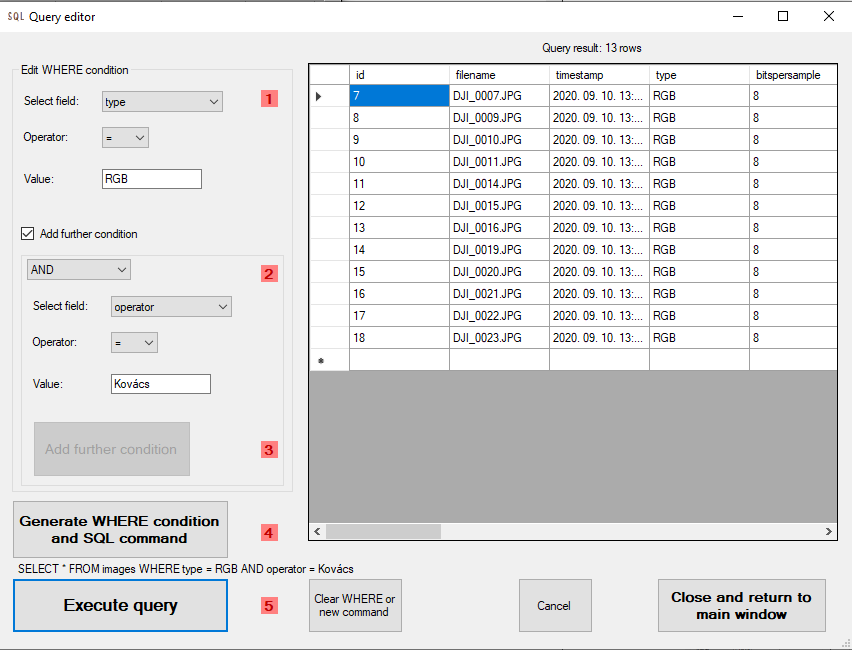
\includegraphics[width=12cm]{sqleditor.png}
	\caption{The \textit{Sql editor} window}
	\label{fig:sqleditor}
\end{figure}

The 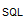
\includegraphics [width = 0.5cm] {sql.png} icon can be used to compile SQL commands to search (collect) according to the parameters of the available images. Fig. \ref {fig:sqleditor}. shows the result of collecting where images were taken on Tisza river and the image type is 'multispectral'. The 'Sql editor' is for those users who do not know Sql language or only at a basic level.
(For users familiar with Sql, a hidden Sql command line can be invoked by pressing F12 key. It is hidden because it can be a dangerous weapon in the hands of those who are unfamiliar with Sql, since it can cause serious damage to the database. Not only queries but also non-query commands can be executed. The command can be executed with \textbf {Enter}.) Command line can be removed by pressing F12 again.

Use the 
\includegraphics [width = 0.5 cm] {sheet.png} icon to view or create a report file for storing specific information on the measurement including data that we find interesting due to the measurement conditions or in any way. 

Clicking to the icon 
\includegraphics{mapviewer_ikon.png} you can see the centroids of selected images on a map background. Map providers can be changed from Google maps to Bing maps.

\subsubsection{Query editor}

\begin{itemize}
	\item  Clicking on the icon 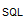
\includegraphics {sql.png} will bring up a window called 'Query editor'. Here you can choose which field to ask, what condition to impose. 
	
	\item e.g. select field: 'type'; Operator: '='; Value: 'RGB' $\rightarrow$ WHERE type = 'RGB'. When done, click on 'Generate WHERE condition and Sql command' then 'Execute query'. 
	
	\item If there is a new query, click on 'Clear WHERE or new command' first. Caution, the Sql editor case sensitive (rgb! = RGB) 
	
	\item For more complex queries, after a query similar to the previous one, click on the check box called 'Add further condition'.  
	
	\item When you are done with a further condition, click on the 'Add further condition' button. If you added the last one, click on 'Generate WHERE condition and Sql command' and then on 'Execute query'. If the sql command was good, the result is displayed in the data grid. 
	
	\item When you are satisfied with the result, click on the 'Close and return to main window' button. The 'Query editor' window will close and the result of the query will be displayed in the main window. Here you can view the list of images. 
	
	\item By clicking on the button labeled 'Select all' with the left mouse button we can collect all the images from the database, the data of which will also appear in the data grid. 
	
	\item By right-clicking on the button labeled 'Select all', you can select all the images in the data grid (fig. \ref {fig:mapviewer}.). This is useful when you want to display the centroids of the collected images on a map. To do this, click on the  
\includegraphics [width = 0.5 cm] {mapviewer_ikon.png} icon. The centroids of the images will then appear in the 'Map viewer' window (fig. \ref {fig:mapviewer}). If we clicked on the 
\includegraphics [width = 0.5 cm] {mapviewer_ikon.png} icon without selecting any images, the location of the ELTE Institute of Map Science and Geoinformatics will appear on the map (fig. \ref {fig:mapviewer}. bottom part). 
	
	\item Clicking on the button labeled 'Select all' will display all records in the data grid with the left mouse button. This overwrites the collection results of the 'Query editor', i.e. the data grid is reset. However, if you right-click this button, all records will be selected in the data grid. If you then click on the ico 
\includegraphics [width = 0.5 cm] {mapviewer_ikon.png}, the selected records will appear in the map window.
	
%	\begin{figure}
%	\centering
%	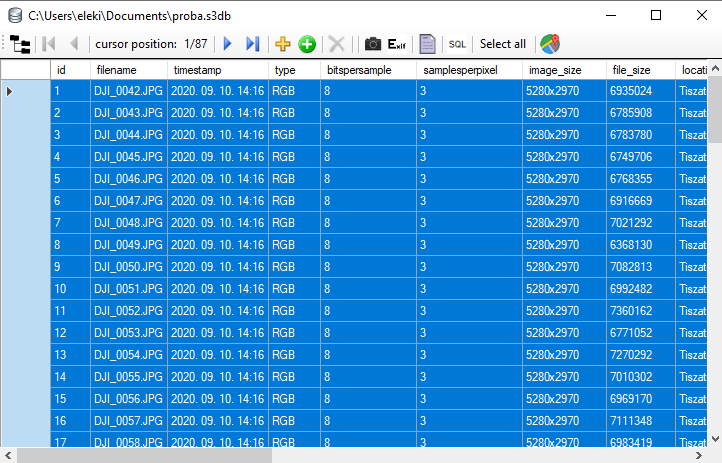
\includegraphics[width=12cm]{mapviewer_select_all.png}
%	\caption{The \textit{Map viewer} window}
%	\label{fig:mapviewer_select_all}
%	\end{figure}

\begin{figure}
	\centering
	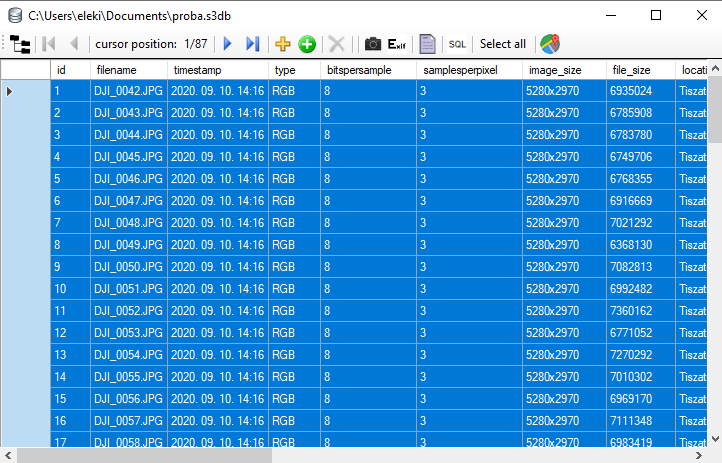
\includegraphics[width=10cm]{mapviewer_select_all.png}
	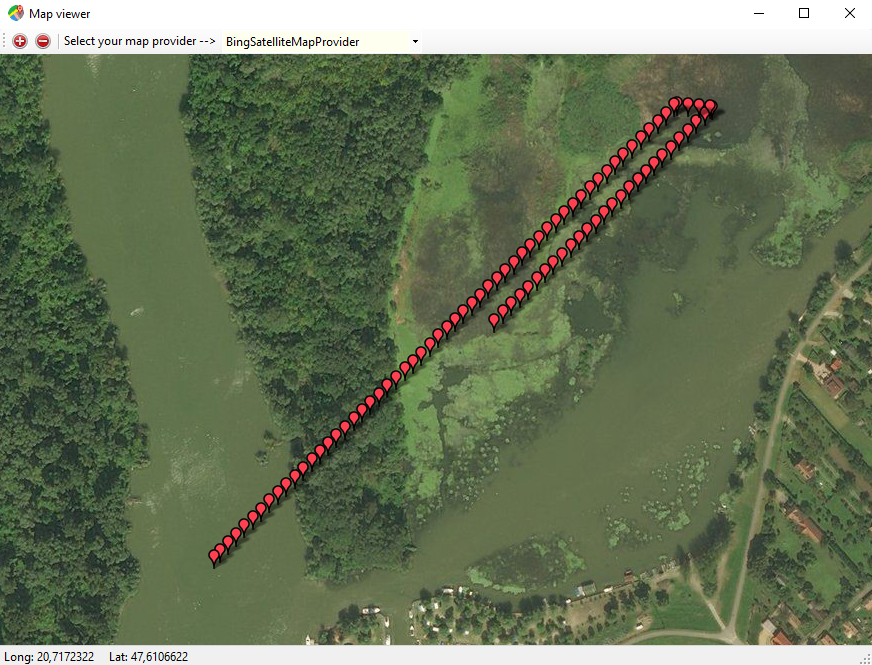
\includegraphics[width=10cm]{mapviewer.png}
	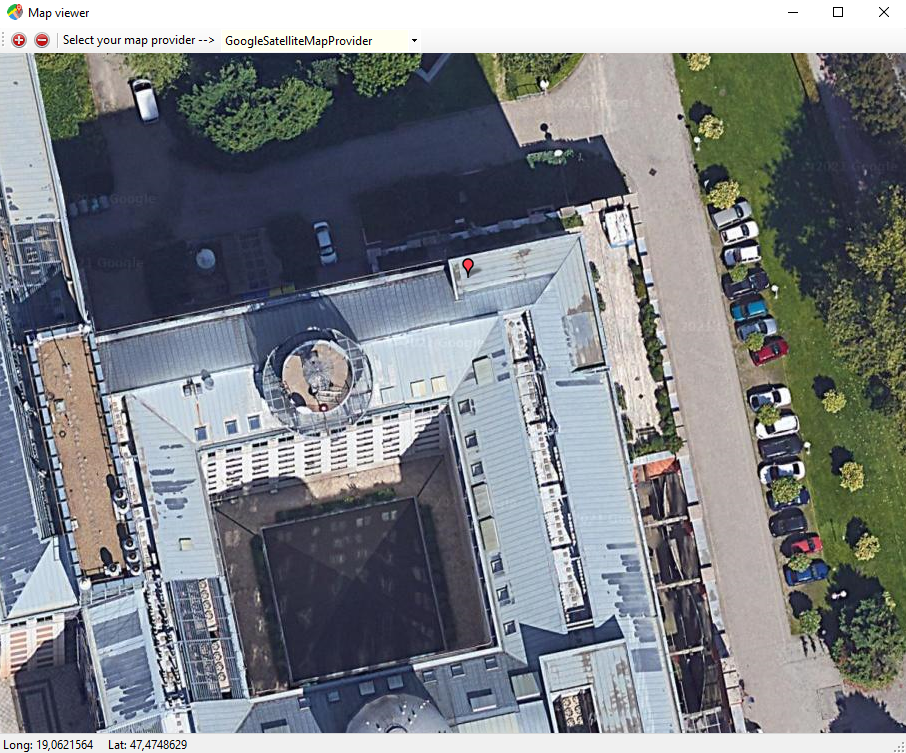
\includegraphics[width=10cm]{tegeta.png}		
	\caption{The \textit{Map viewer} window . The central part shows the Kormoran port (Tiszafured), while the lower part shows the Eotvos Lorand University }
	\label{fig:mapviewer}
\end{figure}
	
	If you click on each record one by one while holding down the CTRL key, they will be selected and shown on the map background. 
	
	
	
\end{itemize}

\section{Data stock}

Data stock is a warehouse where you can select, open, display and analyse your data.  Geotif and bil data can be accessed.  A menu system supports you.   You  can  manipulate  and  display  these  files  in  their  original  format.

Since sometimes really big data files are available, we create an own data format (gwr format) which can be read very fast.  If you have huge files, it is suggested to convert original files to gwr format. Either you have gwr, geotif or bil  files you can use the menu system for doing any computation. The menu system activates the desired funtion from the Giwer’s function library.

\begin{itemize}	
\item Loads images in different formats: gwr, bil, tif, jpg, 8, 16, 24, 48 bits images, from 3-band RGB to 250-band images 
\item Creates an RGB image from any of 3 tracks 
\item Histogram equalisation and drawing 
\item Cross-plot drawing from any of two bands
\item Handling file header (display/edit)
\item Apply functions to process images 
\item NDVI and PCA calculation 
\item Display 3D data with grey-scale, hypsometric or user defined lookup table
\item Raster calculator: querying according to any condition  
\item Combine images (add, average, exor, subtract, etc.)
\item Conversion between formats 
\item Classification methods 
\item Filter bank with many filter methods
\end{itemize}



\subsection{Menus}

When you start \textbf{DataStock} you will see the main menu (fig. \ref{fig:datastock_mainmenu}). The menu system consists of \textit {File}, \textit {One band processes}, \textit {Multiband processes}, \textit {Data tools}, \textit{Workflow} and indicates the current lookup table (available: default, hypsometric, ndvi, user, etc.) that can be changed to another as needed. The \textit {default} option performs greyscale rendering. \textit {hypsometric} allows an 8-bit colouring of up to 256 colours, depending on how many colours are set in the \textit {lookup table}. This is the style of the traditional hypsometric display, which displays low areas with shades of green, slightly higher areas with shades of yellow, and high areas with shades of brown. \textit {ndvi} allows the colour rendering used in the ndvi calculation. \textit {User} sets the \textit {lookup table} set by the user. 

\begin{figure}
	\centering
	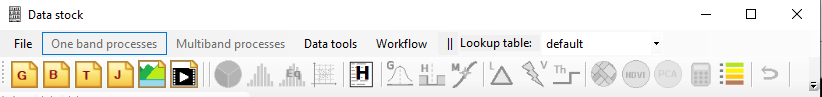
\includegraphics[width=14cm]{datastock_mainmenu.png}
	\caption{The main menu of \textbf{DataStock}}
	\label{fig:datastock_mainmenu}
\end{figure}


\subsubsection{File}

With the \ textit {File} menu (fig. \ref {fig:filemenu_datastock}) you can open \ textit {gwh, bil, tif, jpg} files as well as project files that can handle multiple images at once. You can delete one (or more) \textit {gwh} files. The \textit {gwh, gwr} files are the \textbf {Giwer} system's own format files. You can save the result of a processing in giwer format or as a simple bitmap. You can also save as a project the status of the data in \textbf {Giwer} that currently exists. Finally, we can reload the system configuration data if we have changed it in the meantime with the framework (it does not update automatically). 

\begin{figure}
	\centering
	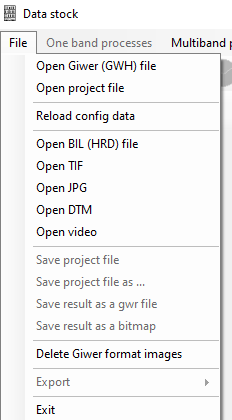
\includegraphics[width=4cm]{filemenu_datastock.png}
	\caption{The \textbf{File} menu}
	\label{fig:filemenu_datastock}
\end{figure}

Selecting images for loading is not yet a display because it may have multiple bands. To do this, select the frequency band you want to display by clicking on one of the list items on the \textit {Layers} tab of the  \textit {Data stock} window (fig. \ref {fig:layer_list}). Once selected, the desired band is displayed and the most menu items and icons (below the main menu) become active. 

\begin{figure}
	\centering
	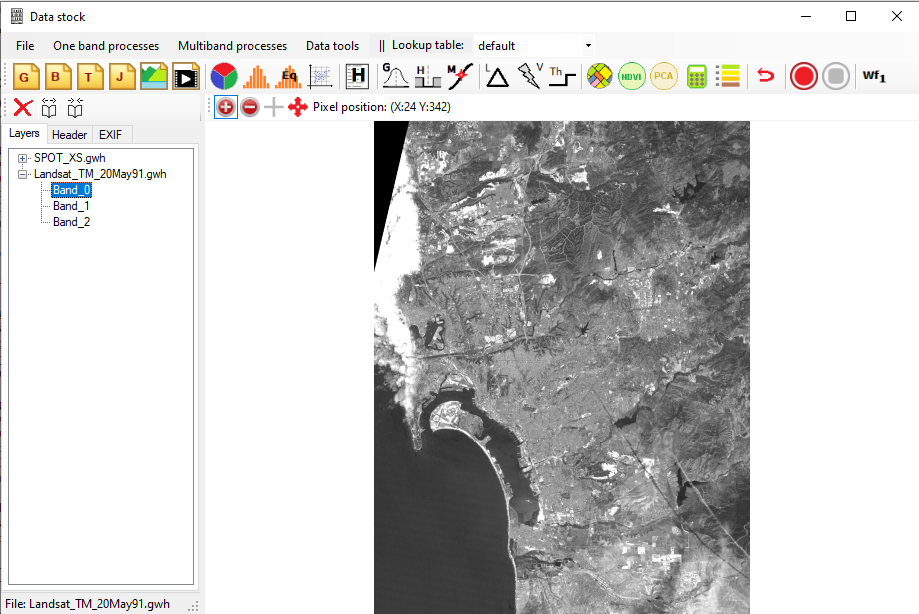
\includegraphics[width=14cm]{layer_list.png}
	\caption{Display images by selecting an item from the \textit {Layer list} }
	\label{fig:layer_list}
\end{figure} 

\textit {gwh} is a text file that contains header-type data about the image (width, height, number of frequency bands, bit depth, etc.), while \textit {gwr} is a binary file that contains pixel data continuously.

The \textit {bil} file is an old space imagery format that also consists of a header file and a binary file. The * .hdr file contains image meta-data and * .bil contains pixel data. A detailed description can be found at \newline \textit {http://desktop.arcgis.com/en/arcmap/10.3/manage-data/raster-and-images/ bil-bip-and-bsq-raster-files.htm}. 
The \textit {tiff} and \textit{jpg} files are well-known image formats that can store images with different colour depths and band numbers. 

The iconostasis below the menu bar shows icons for opening the most common file types, such as \includegraphics [width = 0.5cm] {opengiwer.png} (open giwer format), \includegraphics [width = 0.5cm] {openbil.png} (open bil format), \includegraphics [width = 0.5cm] {opentif.png} (open tif format), \includegraphics [width = 0.5cm] {openjpg.png} (open jpg format), 
\includegraphics [width = 0.5cm ] {3d.png} (open 3D) and \includegraphics [width = 0.5cm] {openvideo.png} (open video). 


\subsubsection{One band processes}

This menu can be used when you want to perform operations on a selected frequency band. After selection, it also appears in the image window.
The elements of the \textit {One band processes} menu are the followings: \textit {Histogram, Thresholding, Vectorising, Filters, Texture, Segmentation, Clustering, Raster calculator} (fig. \ref {fig:onebandmenu}). 

\begin{figure}
	\centering
	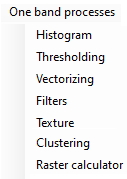
\includegraphics[width=4cm]{onebandmenu.png}
	\caption{The \textbf{One band processes} menu}
	\label{fig:onebandmenu}
\end{figure}

\begin{itemize}	
	\item A \textit{Create RGB} menu creates an RGB image from the three specified frequency bands 
	
	\item A \textit{Segmentation} menu segments to the selected frequency bands.
	
	\item A \textit{Clustering} menu classifies the selected frequency bands.
	
	\item A \textit{PCA} menu performs principal component analysis for the selected frequency bands 
	
	\item Az \textit{NDVI} menu calculates a vegetation index from the selected frequency bands .
	
	\item A \textit{Cross plot} menu draws a cross plot from the two selected frequency bands .
	
	\item A \textit{Combine current image with...} combines the current image (+, -, EXOR) with any other image. This is useful, for example, if you want to draw a vectorized image with the original image (then use the EXOR operator). 	
\end{itemize}

\subsubsection{Data tools}

The \textit {Data tools} menu contains functions for preparing data (fig. \ref {fig:datatools_menu}). It converts, merges and combines different formats. It solves some of the problems with drone images, such as merging multiple image files into a single giwer image, and restoring the align errors of each frequency band. It also allows you to edit \textit {Lookup table}. However, its most important function is the \textit {Convert to Giwer format} submenu. It allows you to convert any raw image format (bil, tif, jpg) to giwer format.

The giwer format means two types of files: \textit {.gwr} is a binary file that contains the image per frequency band, and \textit {.gwh} contains the image header information. 

\begin{figure}
	\centering
	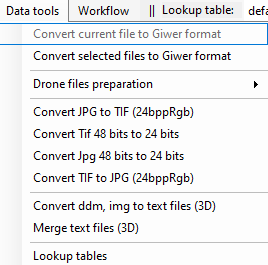
\includegraphics[width=5cm]{datatools_menu.png}
	\caption{The \textit{Data tools} menu}
	\label{fig:datatools_menu}
\end{figure}


The \textit {Convert to Giwer format} menu is only active if an image in tif, jpg or bil format is selected in the list on the \textit {Layers} tab. Clicking this menu will perform the conversion and create the converted data in the location specified in the \textit {Config} file (GiwerDataFolder). Then, by opening this file, the full functionality of \textit {Data Stock} is available. For other image formats, processing operations cannot be activated, only for \textit {giwer} formats.

The \textit {Drone files preparation} menu is used to format certain images. The Micasense multispectral camera, which has 3 RGB and 2 infrared bands as well as one thermal band, produces as many tif files as there are bands, in this case 6 tif files. If you want to convert these to gwr format, you have two options, which are allowed by two submenus: 

\begin{itemize}
	\item Clicking on the \textit {Merge multiple images to giwer format} menu will bring up a dialog box where you can select the files you want. The conversion process then starts, resulting in one \textit {GWH} file and 6 \textit {GWR} files. The header will describe a 6-band image. In any case, this method is recommended because the \textit {Multiband processes} processing processes only work for such files. 
	
	\item Clicking on the \textit {Convert each multiple image to giwer format} menu will bring up a dialog where you can select the files you want. The conversion process then starts, resulting in 6 \textit {GWH} files and 6 \textit {GWR} files. This way, each track will look like a single-track image. Only the \textit {One band processes} menu functions will work on these. 
\end{itemize}

\subsubsection{Some useful functions}

After the main function groups, we also describe some smaller, more convenience functions. Below the menu bar is an iconostasis that provides faster access to certain functions from the menu system: \\

\includegraphics [height = 0.55cm] {ikonosztaz.png} \\ 
From left to right, the following functions are available: open gwr, bil, tif, jpg and video files, take an RGB image, two types of histogram operations where the first is interactive, and also displays the histogram, the other is automatic. Cross plot plotter displays data from two frequency bands on a graph. The icon labeled \textbf {H} hides / shows the header data.

The G icon initiates Gaussian smoothing, H the high pass filter, M the median filter, L the Laplace filter, and Th the thresholding. Then comes the classification icon, then the NDVI calculator, the principal component analysis (PCA), then the raster calculator, and finally the Lookup table editor. The red back arrow \textit {undo} function, ie restores the state before the last operation (only one step back is possible). The big red buttons are used for workflow editing.

The \textit {Layers} tab has three icons: 
\includegraphics [height = 0.55cm] {layer_list_icons.png}. The red cross clears the entire layer list. The book that opens opens a list of frequency bands for all the images in the list, while the book that closes them. To delete only one item from the list, right-click on the desired list item and select delete from the pop-up menu

\subsubsection{Examples}

%	\begin{figure}
%	\centering
%	\includegraphics[width=12cm]{.png}
%	\caption{}
%	\label{fig:}
%	\end{figure}

	\begin{figure}
	\centering
	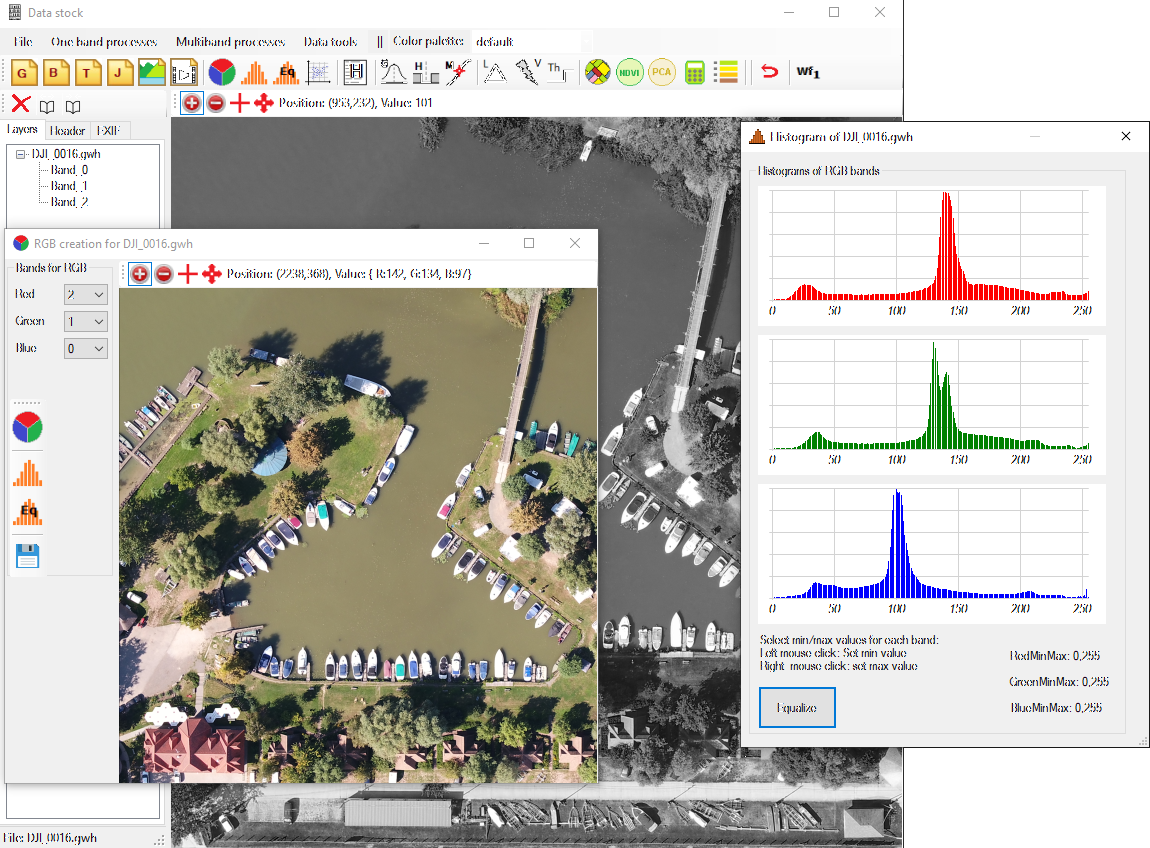
\includegraphics[width=12cm]{gw1.png}
	\caption{Greyscale, RGB and histogram display}
	\label{fig:gw1}
	\end{figure}

	\begin{figure}
	\centering
	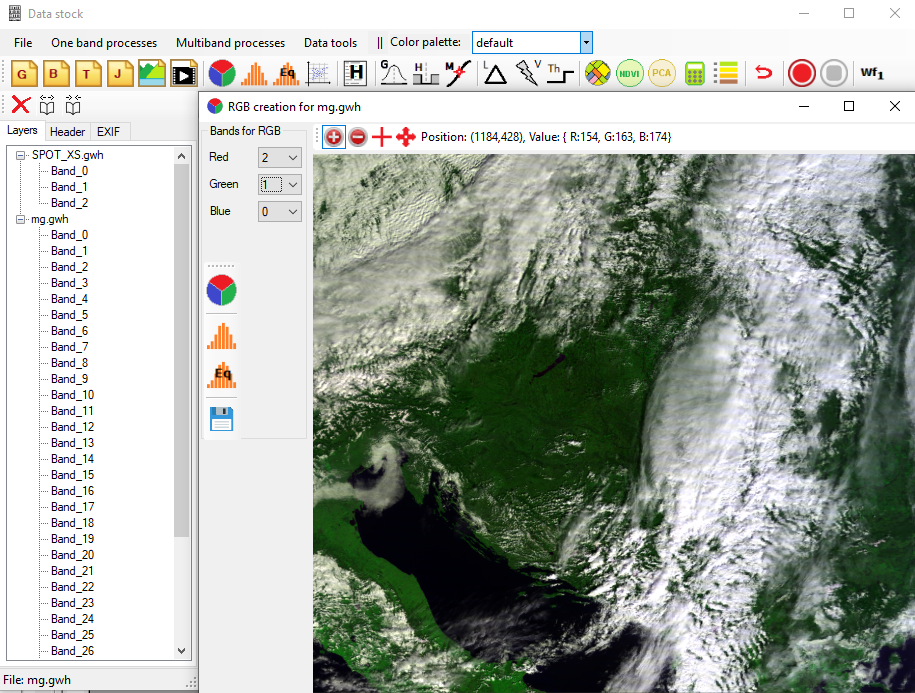
\includegraphics[width=12cm]{ds1.png}
	\caption{RGB  from a hyperspectral image}
	\label{fig:ds1}
	\end{figure}

	\begin{figure}
	\centering
	
\includegraphics[width=12cm]{ndvi.png}
	\caption{RGB versus NDVI}
	\label{fig:ndvi}
	\end{figure}

	\begin{figure}
	\centering
	\includegraphics[width=12cm]{crossplot.png}
	\caption{Crossplot: green band versus red band}
	\label{fig:crossplot}
	\end{figure}

	\begin{figure}
	\centering
	\includegraphics[width=12cm]{pca2.png}
	\caption{The correlation matrix and the first principal component}
	\label{fig:pca2}
	\end{figure}

	\begin{figure}
	\centering
	\includegraphics[width=12cm]{dtm.png}
	\caption{Digital terrain model for Danube band (greyscale and hypsometric shading)}
	\label{fig:dtm}
	\end{figure}

	\begin{figure}
	\centering
	\includegraphics[width=9cm]{cluster.png}
	\caption{Result of clustering}
	\label{fig:cluster}
	\end{figure}

	\begin{figure}
	\centering
	\includegraphics[width=9cm]{cloud.png}
	\caption{A workflow example: detecting a cloud boundary}
	\label{fig:cloud}
	\end{figure}

	\begin{figure}
	\centering
	\includegraphics[width=10cm]{rastcalc.png}
	\caption{Raster calculation form}
	\label{fig:rastcalc}
	\end{figure}

	\begin{figure}
	\centering
	\includegraphics[width=10cm]{lut.png}
	\caption{View/edit lookup table and colour palette}
	\label{fig:lut}
	\end{figure}

	\begin{figure}
	\centering
	\includegraphics[width=14cm]{aligning.png}
	\caption{Result of align correction for Micasense camera}
	\label{fig:aligning}
	\end{figure}


\section{Workflow builder}

\end{document}